\documentclass[11pt]{article}
\usepackage{amsmath, amssymb, amscd, amsthm, amsfonts}
\usepackage{graphicx}
\usepackage{hyperref}
\usepackage{subfigure}
\usepackage{float}
\usepackage{rotating}
\usepackage{tikz}
\usepackage{xcolor}
\usepackage{listings}
\definecolor{vgreen}{RGB}{104,180,104}
\definecolor{vblue}{RGB}{49,49,255}
\definecolor{vorange}{RGB}{255,143,102}
\lstdefinestyle{verilog-style}
{
    language=Verilog,
    basicstyle=\small\ttfamily,
    keywordstyle=\color{vblue},
    identifierstyle=\color{black},
    commentstyle=\color{vgreen},
    numbers=left,
    numberstyle=\tiny\color{black},
    numbersep=10pt,
    tabsize=4,
    moredelim=*[s][\colorIndex]{[}{]},
    literate=*{:}{:}1
}

\makeatletter
\newcommand*\@lbracket{[}
\newcommand*\@rbracket{]}
\newcommand*\@colon{:}
\newcommand*\colorIndex{%
    \edef\@temp{\the\lst@token}%
    \ifx\@temp\@lbracket \color{black}%
    \else\ifx\@temp\@rbracket \color{black}%
    \else\ifx\@temp\@colon \color{black}%
    \else \color{vorange}%
    \fi\fi\fi
}
\makeatother

\usepackage{trace}



\oddsidemargin 0pt
\evensidemargin 0pt
\marginparwidth 40pt
\marginparsep 10pt
\topmargin -20pt
\headsep 10pt
\textheight 8.7in
\textwidth 6.65in
\linespread{1.2}

\title{Digital Bubble Level}
\author{Vladislav Pomogaev - 26951160}
\date{September 27, 2021}

\newcommand{\rr}{\mathbb{R}}

\newcommand{\al}{\alpha}
\DeclareMathOperator{\conv}{conv}
\DeclareMathOperator{\aff}{aff}

\begin{document}

\maketitle

\section{Introduction}
This device forms a digital bubble level; also called a spirit level. It can be helpful in levelling things horizontally.
\begin{figure}[H]
    \centering
    \subfigure[]{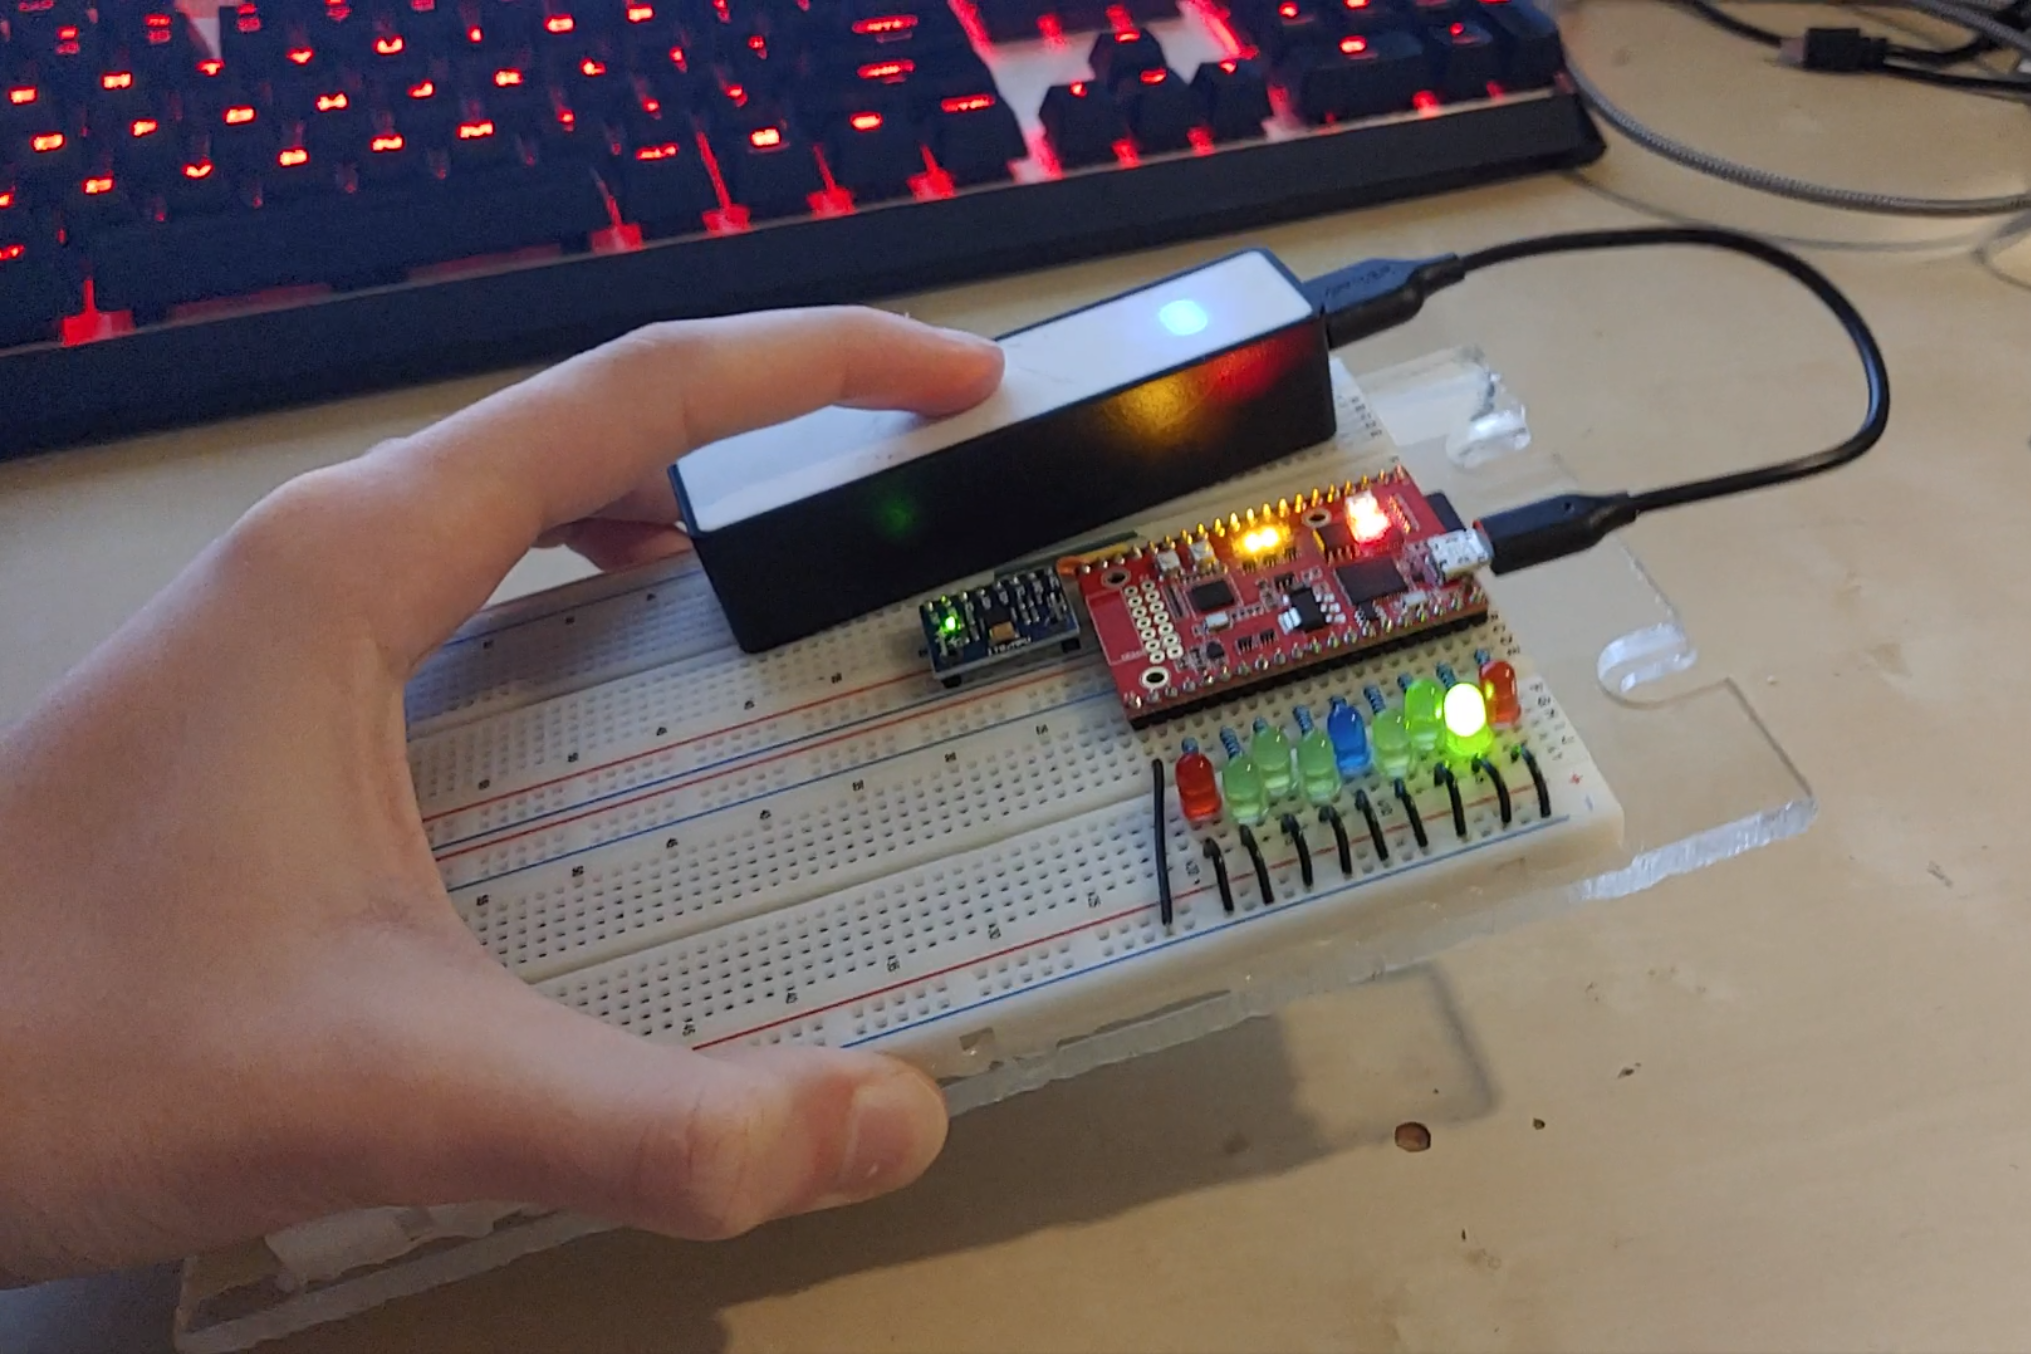
\includegraphics[width=0.32\textwidth]{tilt_1.png}} 
    \subfigure[]{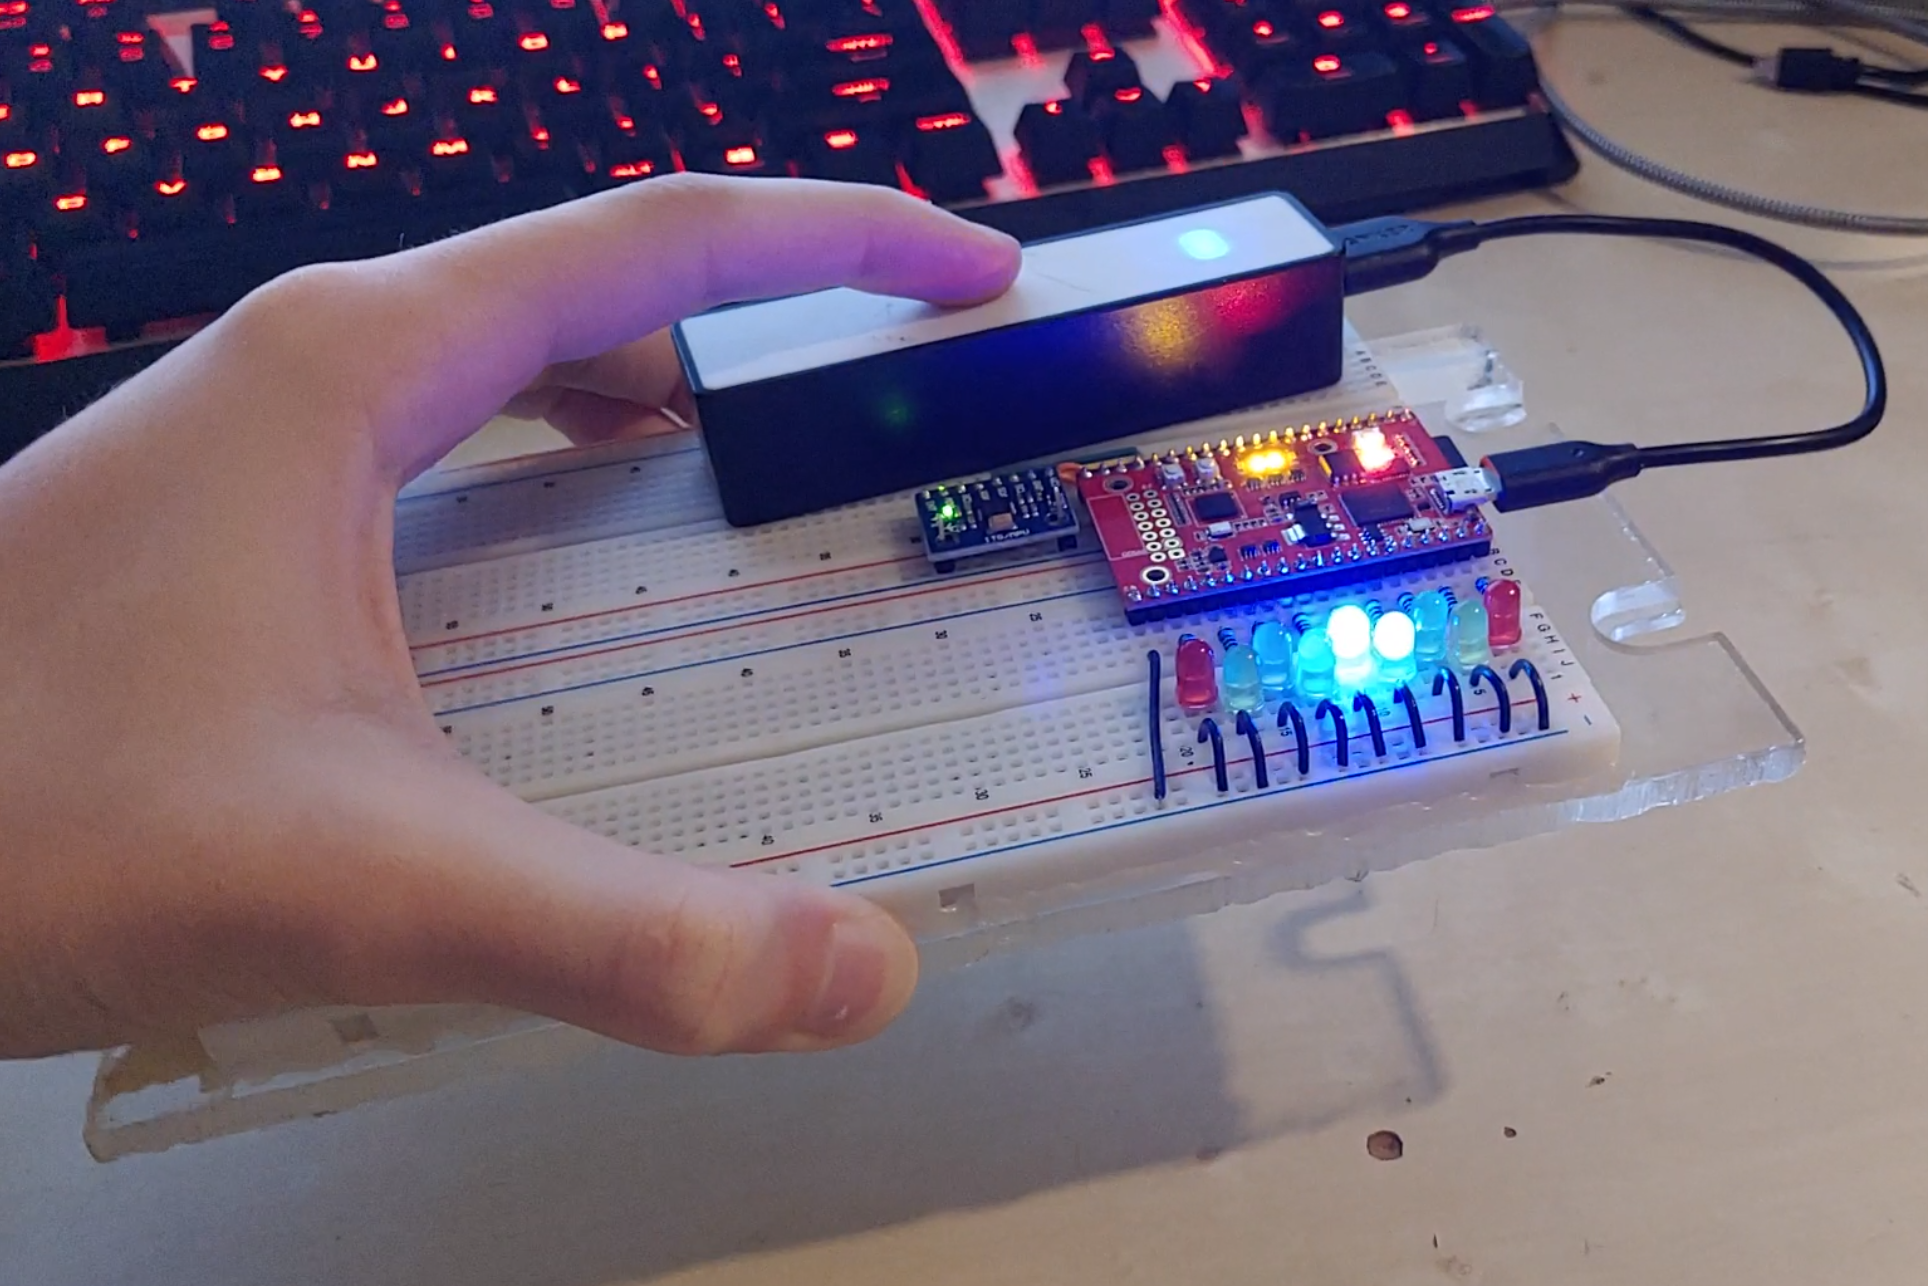
\includegraphics[width=0.32\textwidth]{tilt_3.png}} 
    \subfigure[]{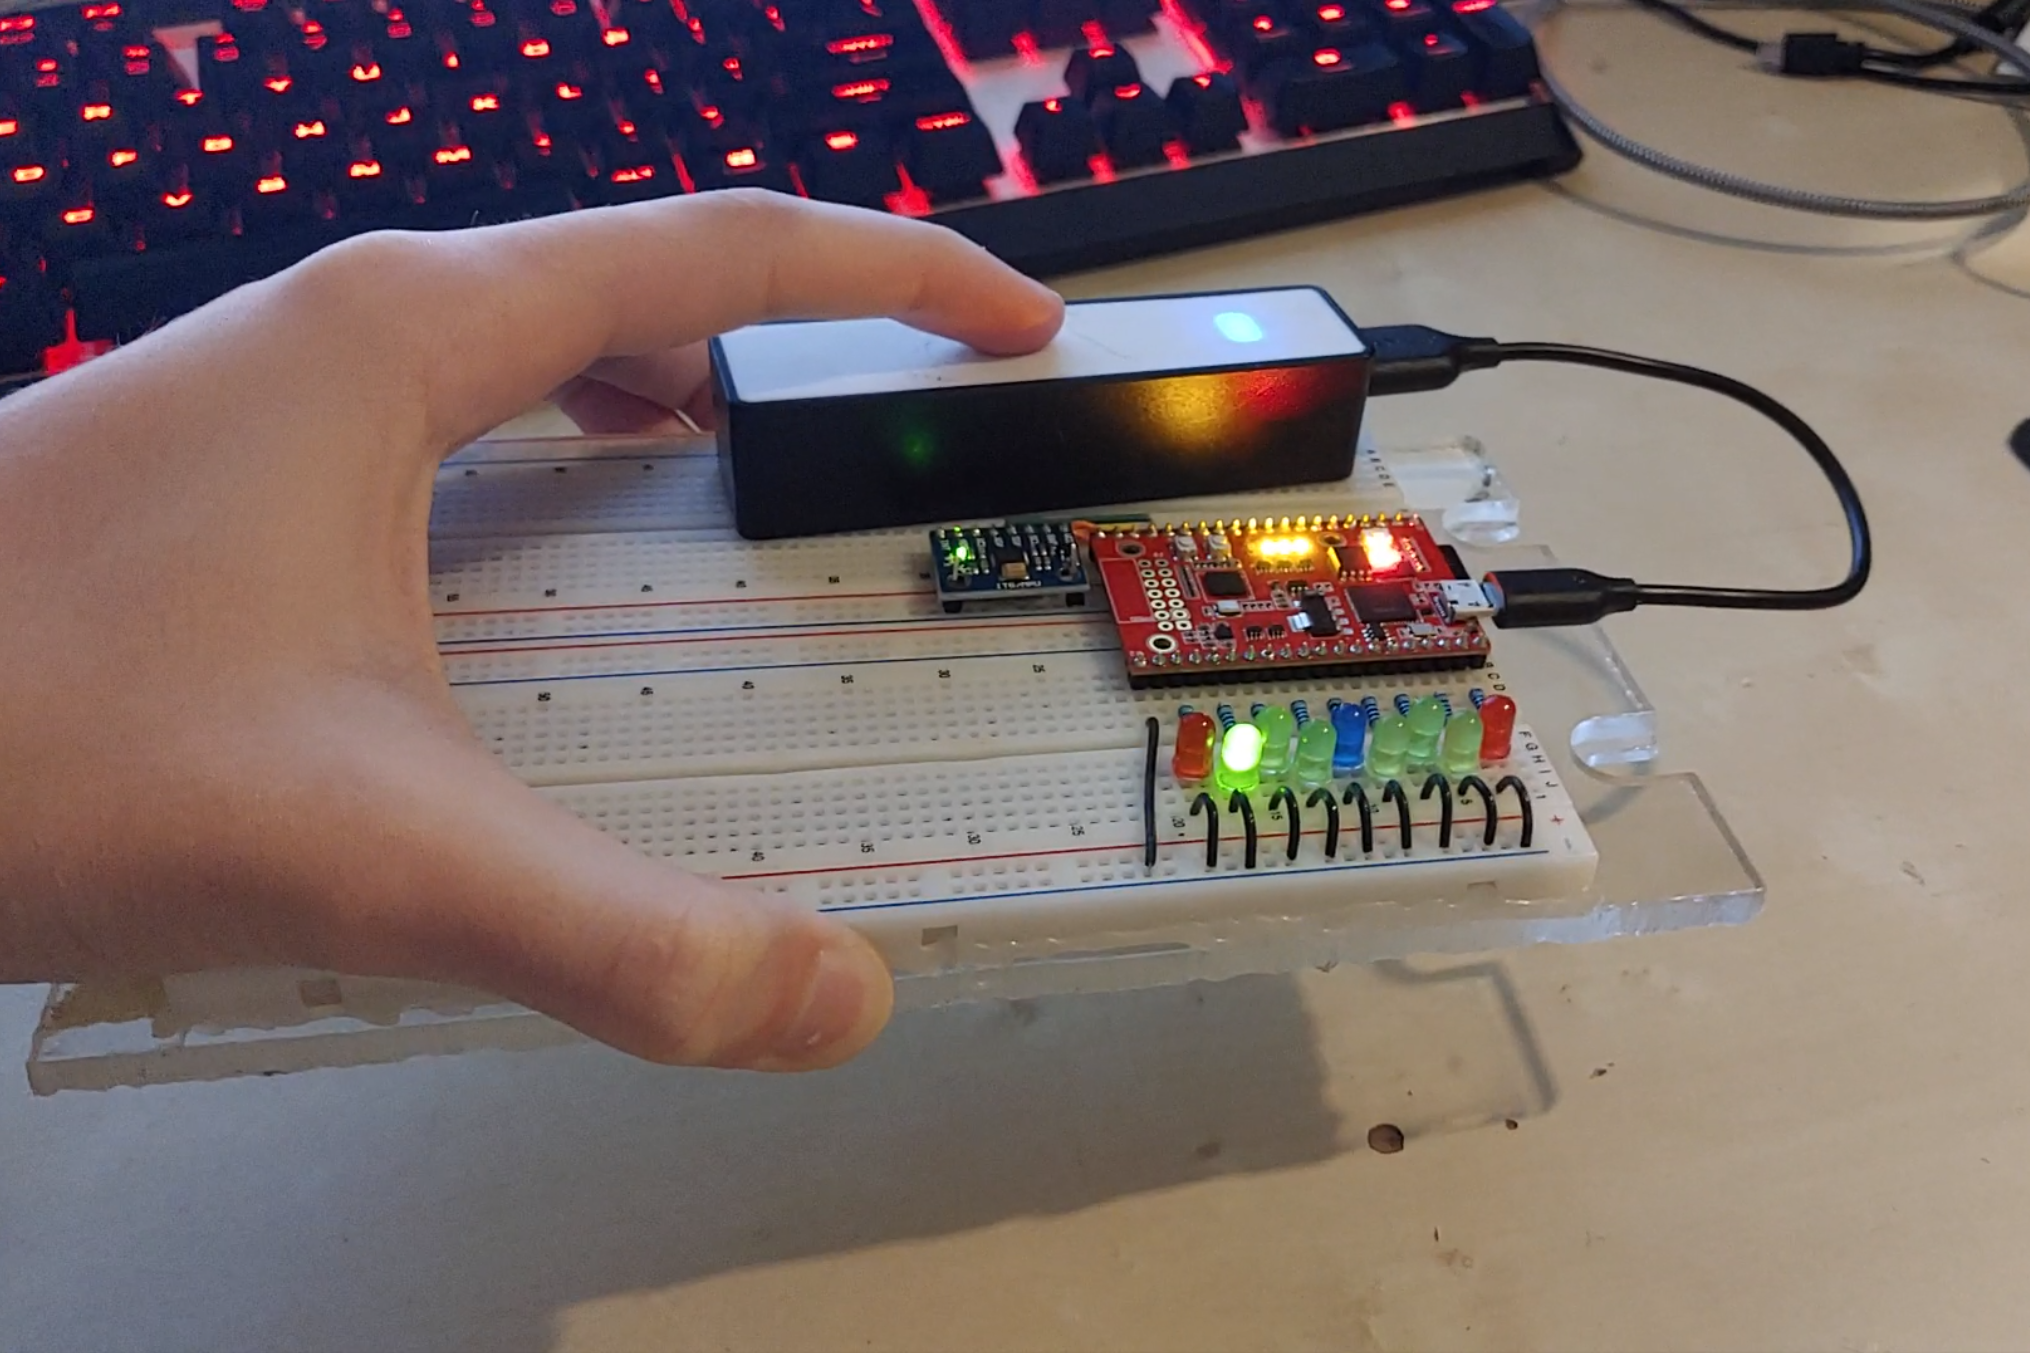
\includegraphics[width=0.32\textwidth]{tilt_2.png}}
    \caption{Photo stills of the device in action. When you tilt the device to the left as in a), the LEDs to the right light up. As you tilt the device more to the right, the lit LED moves from right to left as in b) and c). When level, the blue center LED lights up.}
\end{figure}

This project consists of a synthesised Verilog design running on an Efinix Xyloni FPGA development board. An accelerometer (MPU-6050) and 9 LEDs are connected to this board.

The Verilog design consists of an FSM (Finite State Machine), and an I\textsuperscript{2}C controller IP block from Efinix. The FSM can send commands to the accelerometer through the I\textsuperscript{2}C controller, which acts as the master. Upon reset, the FSM wakes the accelerometer by writing to a register. Then, in a loop, the FSM requests the acceleration measured in one axis from the accelerometer, and converts the acceleration to a grey-code-like signal which is then output to the LEDs. All of this is done while implementing the communication protocol of the I\textsuperscript{2}C controller. The FSM must request data in the correct format, provide slave address, data, command byte, and number of data bits, wait for response, and check for errors during every read and write command.

\section{Overview}
\begin{figure}[H]
    \centering
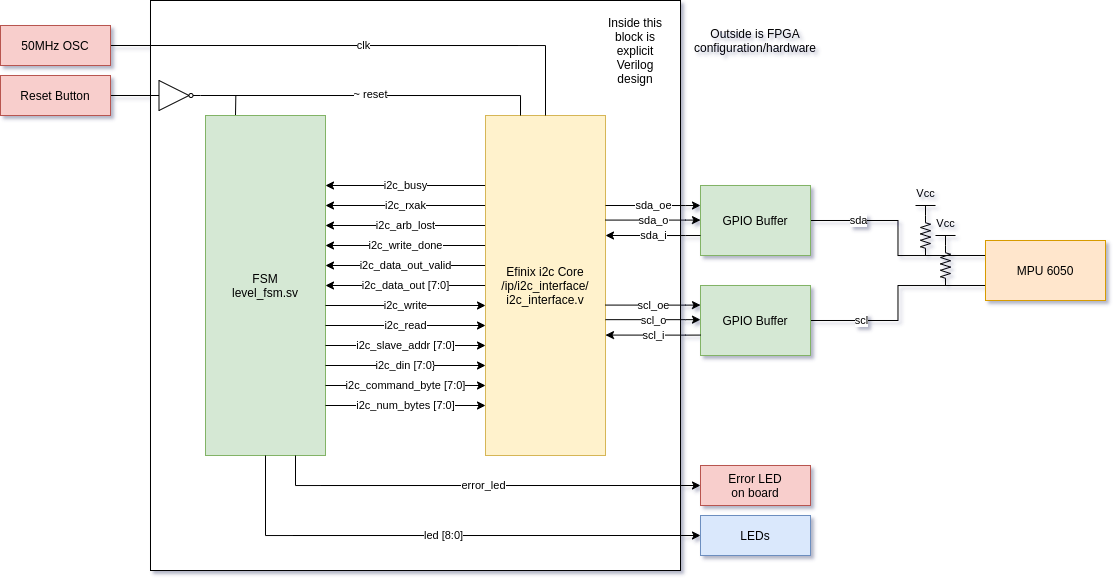
\includegraphics[width=0.99\textwidth]{fsm.png}
    \caption{Block diagram of the FSM and how it forms the bubble-level system. The level FSM talks to the I2C core, which communicates to the MPU via a set of buffered GPIO blocks on the FPGA. A reset button resets all FSMs to their initial state. The design runs is compiled for a 50MHz clock constraint. The output to outside of the FPGA is buffered through the GPIO logic blocks, which was the reason I used IP specific to the FPGA.}
\end{figure}

\begin{figure}[H]
    \centering
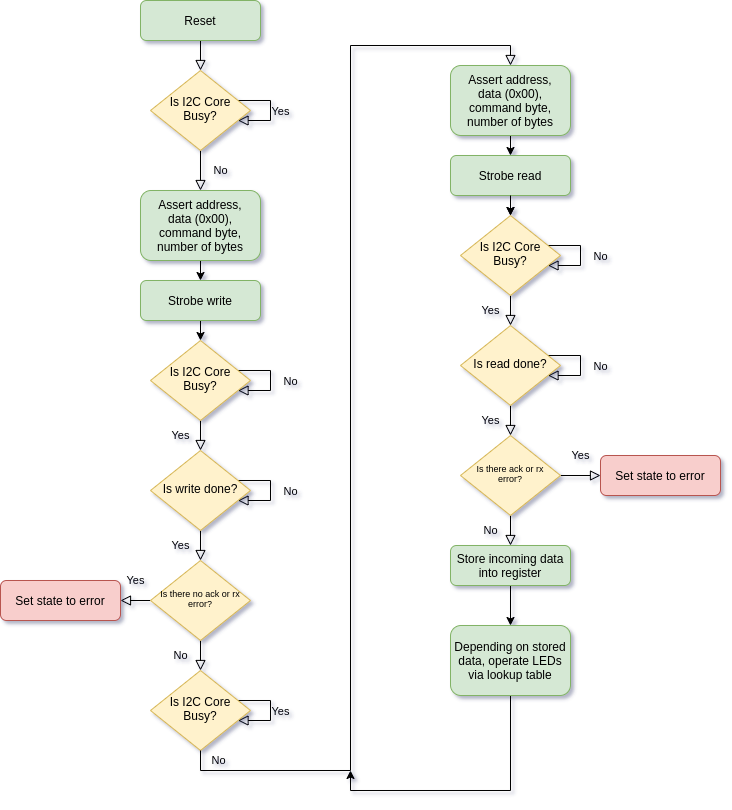
\includegraphics[width=0.99\textwidth]{flow.png}
    \caption{Flow diagram of the internal functioning of the FSM. The assertion of the addresses, data, command byte is done even though it is slightly redundant in this situation to allow for easy expansion of functionality by changing those lines to be tri-state and allowing other modules to write to them.}
\end{figure}

\begin{figure}[H]
    \centering
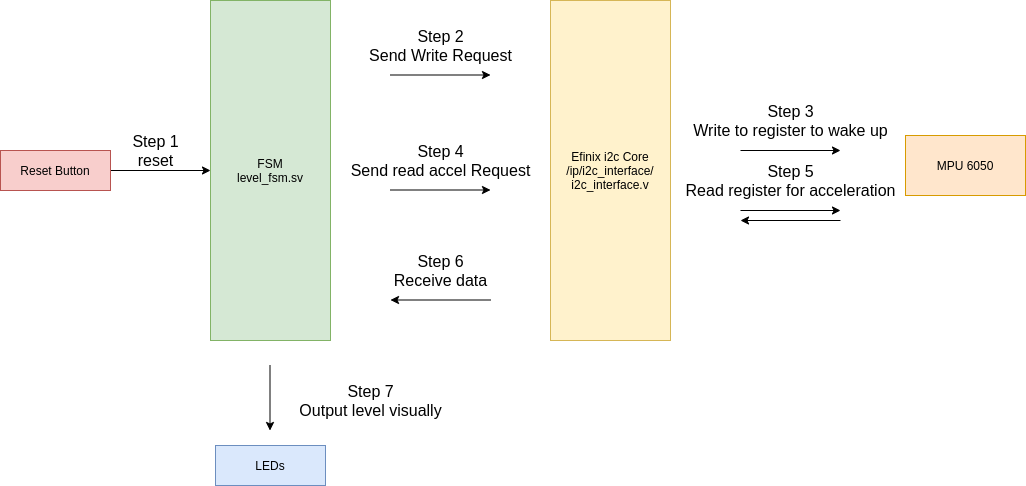
\includegraphics[width=0.99\textwidth]{data_flow.png}
    \caption{Data flow diagram for the FSM.}
\end{figure}

\subsection{States}
The states for the FSM and their purposes are as follows:

\begin{lstlisting}[style={verilog-style}, basicstyle=\tiny,]
typedef enum logic [6:0] { 
  ENSURE_BUSY_1 =      7'b0000_000, // wait for I2C controller to not be busy
  ASSIGN_WRITE_2 =     7'b0001_000, // tell I2C controller which registers to write what to
  ASSERT_WRITE_3 =     7'b0010_001, // tell I2C controller to write
  WAIT_FOR_BUSY_4 =    7'b0011_000, // wait for controller to be busy
  WAIT_FOR_DONE_5 =    7'b0100_000, // wait for controller to finish
  VERIFY_6 =           7'b0101_000, // verify that there were no errors writing register
  ENSURE_BUSY_7 =      7'b0110_000, // verify that the controller is not busy
  ASSIGN_WRITE_8 =     7'b0111_000, // tell I2C controller which registers to read
  ASSERT_READ_9 =      7'b1000_010, // tell I2C controller to read register
  WAIT_FOR_BUSY_10 =   7'b1001_000, // wait for controller to be busy
  WAIT_FOR_VALID_11 =  7'b1010_000, // wait for controller to finish read
  VERIFY_12 =          7'b1011_000, // verify that no errors occured, register info
  LED_OPERATION_13 =   7'b1100_000, // output LED pattern
  ERROR =              7'b1101_100
} state_e;

\end{lstlisting}

\section{Testing}


\begin{figure}[H]
    \centering
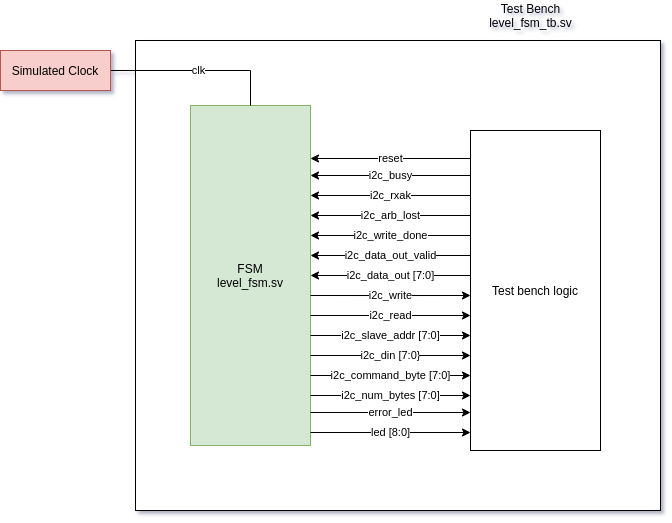
\includegraphics[width=0.99\textwidth]{tb.png}
    \caption{Block diagram of how the level FSM (not the Efinix i2c core) is connected to the test bench. The test bench is a simple piece of logic that provides timed inputs to the level FSM and asserts that the outputs of the FSM are what are expected. When a new test is run by the test bench logic, the instantiated DUT is reset. Asserts are used to check correct functionality. }
\end{figure}

The I2C core provided by Efinix was autogenerated and came with it's own test-bench. Since I did not write this IP or the test bench, I do not include the source code for this report nor diagrams for it. I'm taking it at face-value and trusting that it works.


\begin{sidewaysfigure}
    \centering
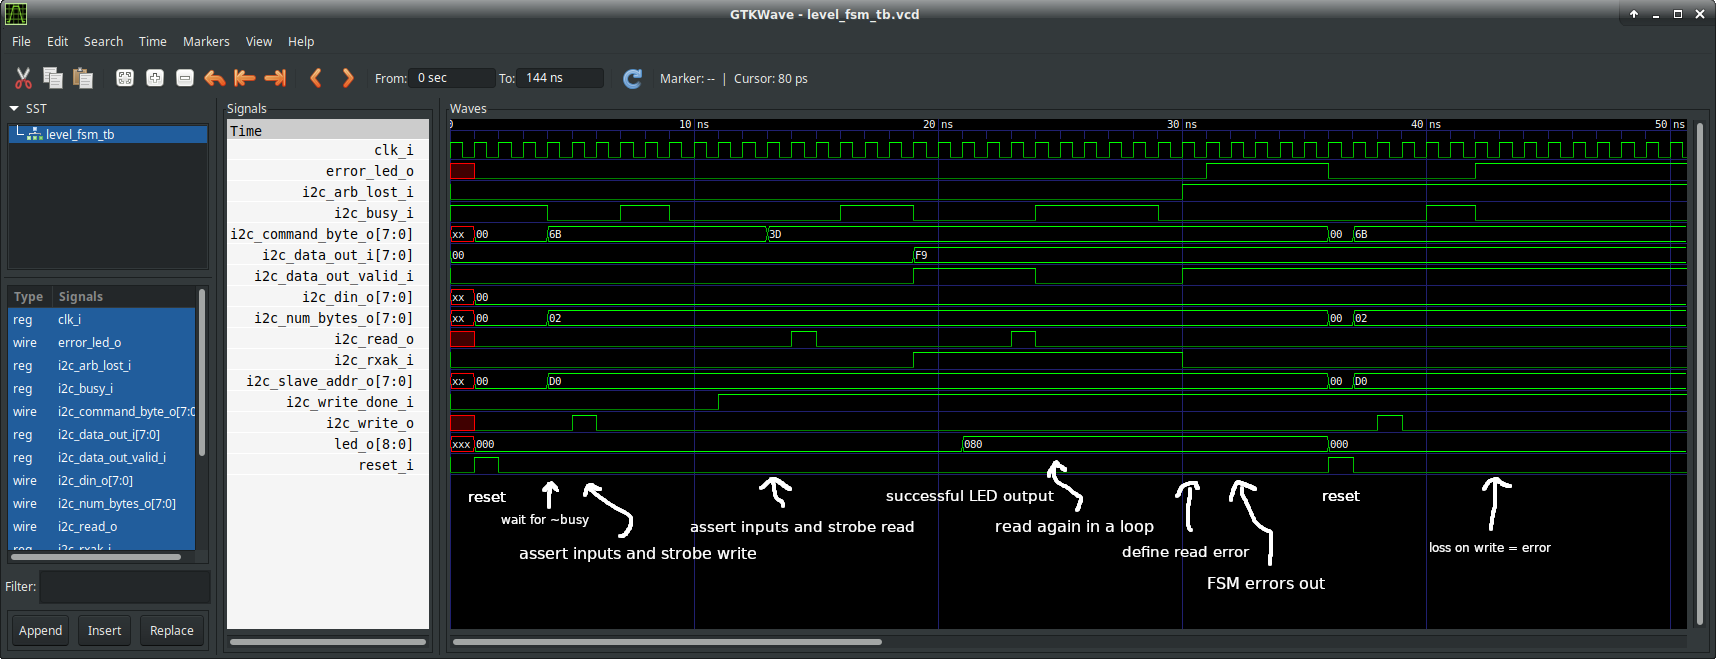
\includegraphics[width=0.99\textwidth]{waveform2.png}
    \caption{Waveform diagram from FSM test. The FSM was tested under three scenarios: perfectly functioning I2C controller and MPU, an error on the read command, and an error on the write command. All delays were verified to work (waiting for busy, write and read finish). }
\end{sidewaysfigure}

\pagebreak
\section{Code (also included in separate file)}
level{\_}fsm.sv
\lstinputlisting[style={verilog-style}, basicstyle=\tiny,]{level_fsm.sv}
level{\_}fsm{\_}tb.sv
\lstinputlisting[style={verilog-style}, basicstyle=\tiny,]{level_fsm_tb.sv}

\end{document}